\documentclass[11pt]{article}

% Paquetes
%===================================================================================================

% Establecemos los márgenes
\usepackage[a4paper, margin=1in]{geometry}

% Separacion entre parrafos
\setlength{\parskip}{1em}

% Paquete para incluir codigo
\usepackage{listings}

% Paquete para incluir imagenes
\usepackage{graphicx}
\graphicspath{ {./images/} }

% Para fijar las imagenes en la posicion deseada
\usepackage{float}

% Para que el codigo acepte caracteres en utf8
\lstset{literate=
  {á}{{\'a}}1 {é}{{\'e}}1 {í}{{\'i}}1 {ó}{{\'o}}1 {ú}{{\'u}}1
  {Á}{{\'A}}1 {É}{{\'E}}1 {Í}{{\'I}}1 {Ó}{{\'O}}1 {Ú}{{\'U}}1
  {à}{{\`a}}1 {è}{{\`e}}1 {ì}{{\`i}}1 {ò}{{\`o}}1 {ù}{{\`u}}1
  {À}{{\`A}}1 {È}{{\'E}}1 {Ì}{{\`I}}1 {Ò}{{\`O}}1 {Ù}{{\`U}}1
  {ä}{{\"a}}1 {ë}{{\"e}}1 {ï}{{\"i}}1 {ö}{{\"o}}1 {ü}{{\"u}}1
  {Ä}{{\"A}}1 {Ë}{{\"E}}1 {Ï}{{\"I}}1 {Ö}{{\"O}}1 {Ü}{{\"U}}1
  {â}{{\^a}}1 {ê}{{\^e}}1 {î}{{\^i}}1 {ô}{{\^o}}1 {û}{{\^u}}1
  {Â}{{\^A}}1 {Ê}{{\^E}}1 {Î}{{\^I}}1 {Ô}{{\^O}}1 {Û}{{\^U}}1
  {ã}{{\~a}}1 {ẽ}{{\~e}}1 {ĩ}{{\~i}}1 {õ}{{\~o}}1 {ũ}{{\~u}}1
  {Ã}{{\~A}}1 {Ẽ}{{\~E}}1 {Ĩ}{{\~I}}1 {Õ}{{\~O}}1 {Ũ}{{\~U}}1
  {œ}{{\oe}}1 {Œ}{{\OE}}1 {æ}{{\ae}}1 {Æ}{{\AE}}1 {ß}{{\ss}}1
  {ű}{{\H{u}}}1 {Ű}{{\H{U}}}1 {ő}{{\H{o}}}1 {Ő}{{\H{O}}}1
  {ç}{{\c c}}1 {Ç}{{\c C}}1 {ø}{{\o}}1 {å}{{\r a}}1 {Å}{{\r A}}1
  {€}{{\euro}}1 {£}{{\pounds}}1 {«}{{\guillemotleft}}1
  {»}{{\guillemotright}}1 {ñ}{{\~n}}1 {Ñ}{{\~N}}1 {¿}{{?`}}1 {¡}{{!`}}1
}

% Para que no se salgan las lineas de codigo
% Para fijar una fuente que resalte
\lstset{breaklines=true, basicstyle=\ttfamily}

% Para que los metadatos que escribe latex esten en español
\usepackage[spanish]{babel}
\decimalpoint % Para que no se cambie el punto a la coma

% Para la bibliografia
% Sin esto, los enlaces de la bibliografia dan un error de compilacion
\usepackage{url}

% Para que se puedan clicar los enlaces
\usepackage{hyperref}

% Para mostrar graficas de dos imagenes, cada una con su caption, y con un caption comun
\usepackage{subcaption}

% Simbolo de los numeros reales
\usepackage{amssymb}

% Para que los codigos tengan una fuente distinta
\usepackage{courier}

\lstdefinestyle{CustomStyle}{
  language=Python,
  numbers=left,
  stepnumber=1,
  numbersep=10pt,
  tabsize=4,
  showspaces=false,
  showstringspaces=false
  basicstyle=\tiny\ttfamily,
}

% Para referenciar secciones usando el nombre de las secciones
\usepackage{nameref}

% Para enumerados dentro de enumerados
\usepackage{enumitem}

% Para mejores tablas
\usepackage{tabularx}

% Para poder tener el mismo identificador en dos tablas separadas
\usepackage{caption}

% Mostrar la página de las referencias en el indice del documento
\usepackage[nottoc,numbib]{tocbibind}

% Para mostrar las matrices
\usepackage{amsmath}

% Para que las notas al pie de pagina queden bien abajo
\usepackage[bottom]{footmisc}

% Para poner tablas en horizontal, ocupando bien la página
% cuando hay mucho texto en la table
\usepackage{lscape}

% Comandos personalizados
%===================================================================================================

% Para realizar las citas de forma corta
\newcommand{\customcite}[1]{\emph{"\ref{#1}. \nameref{#1}"}}

% Para entrecomillar un texto
\newcommand{\entrecomillado}[1]{\emph{``#1''}}

% Metadatos del documento
%===================================================================================================
\title{
    {Visión por Computador - Práctica Final} \\
    {Uso de redes siamesas para la clasificación de fotografías de ropa (Zalando)}
}

\author{
    {Sergio Quijano Rey}\\
    {sergioquijano@correo.ugr.es} \\
    {}\\
    {Alejandro Borrego Mejías} \\
    {alejbormeg@correo.ugr.es}\\
}

\date{\today}

% Separacion entre parrafos
\setlength{\parskip}{1em}

% Contenido del documento
%===================================================================================================
\begin{document}

% Portada del documento
\maketitle
\pagebreak

% Indice de contenidos
\tableofcontents

% Lista de figuras
% Uso el addtocontents para que no se muestre la seccion de indice de figuras en el indice inicial

\addtocontents{toc}{\setcounter{tocdepth}{-10}}
\listoffigures

% TODO -- no tenemos cuadros en esta memoria
\listoftables

% TODO -- tampoco tenemos codigos de relevancia
% \lstlistoflistings
\addtocontents{toc}{\setcounter{tocdepth}{3}}

\pagebreak

\section{Introducción}

\subsection{Problema a resolver}

En esta práctica vamos a trabajar con el uso de redes siamesas y la función de pérdida \emph{Triplet Loss}. Por tanto, calcularemos un \emph{embedding} de la base de datos. Adaptaremos dicha red para realizar una tarea de clasificación usando el algoritmo \emph{k-NN}.

Realizaremos dos experimentos. El primero de ellos basado en el entrenamiento de la red usando triples aleatorios. El segundo, basado en el entrenamiento de la red usando triples difíciles, calculados de forma \emph{online} por cada \emph{minibatch}.

\subsection{Elección del \emph{dataset}}

El dataset que hemos utilizado para la realización de este proyecto se denomina \emph{FashionMNIST} \cite{zalando_dataset:online} y nos proporciona un total de 60000 imágenes $28 \times 28$ en escala de grises de ropa de distintos tipos (en concreto de 10 clases distintas). 

Esta base de datos surge como una alternativa al famoso conjunto de datos \emph{MNIST}. Los autores de la base de datos buscaban mantener la estructura de la base de datos original (tamaño de las imágenes, número de clases, tamaños de los conjuntos de entrenamiento y test, \ldots) a la vez que proponer un mayor reto que el reconocimiento de dígitos \cite{database_why:online}.

Más adelante, en \customcite{adecuacion_arquitectura_red:seccion}, discutiremos sobre la ideonidad de la arquitectura de red teniendo en cuenta la base de datos que acabamos de presentar.

\subsection{Motivación} \label{motivacion:seccion}

Hemos elegido este proyecto por nuestro interés en el estudio de redes Siamesas. Queríamos profundizar en su funcionamiento, en concreto, en las dificultades que supone la generación de triples para el correcto entrenamiento de la red a través de la función de error \emph{Triplet Loss}. De hecho, y como comentaremos más adelante, esta ha sido la parte más complicada del proyecto, pues escribir un código lo más eficiente posible ha sido crítico para reducir drásticamente los tiempos de ejecución.

La elección de la base de datos viene motivada por la actualidad de los datos que en ella se presentan y por las características de la misma. En concreto, es una base de datos lo suficientemente sencilla como para permitirnos realizar la experimentación aquí presentada en tiempos razonables, a la vez que tratábamos un problema más o menos complejo de resolver.

\subsection{Objetivos a realizar}

Los objetivos que nos proponemos en este proyecto son: 

\begin{enumerate}
  \item Aplicar \emph{Transfer Learning}. Durante todos los experimentos, usaremos una red \emph{ResNet18} pre-entrenada sobre \emph{ImageNet} que modificaremos ligeramente (en la capa de salida) y sobre la que realizaremos \emph{fine tuning}.
  \item Entrenamiento de la red usando triples aleatorios. Esperamos obtener resultados muy malos. Sin embargo, tomamos esto como \emph{baseline}, con el que compararemos cuando propongamos una mejor forma de tomar los triples con los que entrenamos.
  \item Entrenamiendo de la red usando triples difíciles, calculados de forma \emph{online} dentro de cada \emph{minibatch}. Con esto esperamos obtener una mejora drástica frente al uso de triples aleatorios.
  \item Adaptación de ambas redes (la entrenada con triples aleatorios y la entrenada con triples difíciles) a una tarea de clasificación usando \emph{k-NN} sobre el \emph{embedding} que las redes siamesas calculan.
\end{enumerate}

\subsection{Otros detalles}

Al principio del \emph{Notebook} definimos una variable \lstinline{RUNNING_ENV} que indica en que tipo de entorno nos encontramos. Cuando \lstinline{RUNNING_ENV == "local"}, indicamos que estamos corriendo el \emph{Notebook} en local, y cuando \lstinline{RUNNING_ENV == "remote"} indicamos que estamos corriendo en \emph{Google Colab}. Así podemos controlar las pequeñas diferencias entre estos dos entornos de desarrollo. Principalmente son dos las diferencias:

\begin{itemize}
    \item Cuando corremos en \emph{Google Colab} tenemos que introducir un código de verificación
    \item Las rutas de la carpeta donde guardamos las imágenes son diferentes
\end{itemize}

Además, al estar usando \lstinline{Pytorch} como librería principal, hemos tenido que escribir mucho código para llevar a cabo tareas básicas (como el bucle del entrenamiento, funciones para mostrar el progreso del entrenamiento conforme se está realizando, funciones para evaluar un clasificador, \ldots) Por ello hemos decidido separar el código de la siguiente forma:

\begin{itemize}
  \item Una carpeta \lstinline{lib/} en la que tenemos ficheros \lstinline{.py} con el código básico del que ya hemos hablado
  \item Un \emph{notebook} \lstinline{Notebook.ipynb}, en el que realizamos todo el trabajo interesante. Por ejemplo, aquí definimos todos los hiperparámetros que usamos finalmente, las funciones de pérdida usadas, la forma de calcular los triples, la evaluación del modelo, \ldots
\end{itemize}


\pagebreak

\section{Fundamentos Teóricos} 

\subsection {\emph{Redes Siamesas}}

Una red siamesa es una arquitectura en la que se tienen dos redes idénticas, con el objetivo que, dadas dos imágenes de entidades iguales, obtengan dos representaciones cercanas. Y al revés, dadas dos entidades distintas, se debe obtener dos representaciones distantes.

Al trabajar con dos redes idénticas, lo que realmente manejamos es una única red que calcula representaciones de imágenes pasadas como entrada. Usaremos dicha red para calcular representaciones de pares o triples (en nuestro caso concretro, trabajaremos sobre todo con triples) de imágenes dadas como entrada.

Aclaramos lo que entendemos por representaciones cercanas y distantes. En primer lugar, la red calculará, dada una imagen de entrada $28\times28$, un embedding de la imagen. Esto es, una representación vectorial es un espacio $\mathbb{R}^d$ con $d << 28*28$ (ie. $d = 2$, $d = 4$, \ldots). 

Con esto, dadas dos imágenes $x, y$, sus representaciones $ f_{\theta}(x),  f_{\theta}(y)$ serán cercanas cuando $$|| f_{\theta}(x) - f_{\theta}(y)||_2 \approx 0$$ Del mismo modo serán lejanas cuando $$|| f_{\theta}(x) - f_{\theta}(y)||_2 >> 0$$ 

\pagebreak
\subsection{\emph{Triplet Loss}}

Esta será la función de pérdida que vamos a usar para optimizar nuestra red siamesa. A continuación introducimos el por qué de su uso.

Durante el entrenamiento, la red verá como ejemplos triples. Esto es, triples de la forma \emph{anchor}, \emph{positive}, \emph{negative}. \emph{anchor} será una imagen arbitraria, mientras que \emph{positive} será una imagen de la misma clase que \emph{anchor} y \emph{negative} será una imagen de otra clase. Queremos que la distancia entre ancla y positivo sea pequeña, y entre ancla y negativo sea grande. Por tanto, lo que queremos es:

$$||f_{\theta}(anchor) - f_{\theta}(positive)||^2 \leq ||f_{\theta}(anchor) - f_{\theta}(negative)||^2 $$

luego 

$$||f_{\theta}(anchor) - f_{\theta}(positive)||^2 - ||f_{\theta}(anchor) - f_{\theta}(negative)||^2 \leq 0$$

Para evitar la trivialidad $f_{\theta}(img) = 0; \forall img$ añadimos un margen $\alpha > 0$ de la siguiente forma:

$$||f_{\theta}(anchor) - f_{\theta}(positive)||^2 - ||f_{\theta}(anchor) - f_{\theta}(negative)||^2 + \alpha \leq 0$$

Con esto, definimos una función de pérdida que solo se activará cuando la desigualdad no se mantenga, con lo que:

$$Loss(a, p, n) := max(||f_{\theta}(a) - f_{\theta}(p)||^2 - ||f_{\theta}(a) - f_{\theta}(n)||^2 + \alpha, 0)$$

\pagebreak
\subsection{Adecuación de la arquitectura de red a la base de datos escogida} \label{adecuacion_arquitectura_red:seccion}

Las redes siamesas se han usado sobre todo en tareas de reconocimiento de caras y en verificación de firmas a mano \cite{siamese_wikipedia:online}. Estos dos problemas presentan las siguientes características fundamentales:

\begin{itemize}
  \item La red tiene que distinguir si dos imágenes se corresponden a la misma entidad o no (dos fotografías de dos personas se corresponden a la misma, dos firmas se han realizado por la misma persona)
  \item La red va a ver ejemplos de entidades no vistas durante el entrenamiento. Por ejemplo, tiene que distinguir si dos fotos de personas son de la misma persona, sin haber visto fotografías de esa persona previamente. En modelos de clasificación clásicos la red puede enfrentarse a fotografías nunca vistas, pero de una clase de la que ha visto otras fotografías. Así, esta es una diferencia fundamental con otros modelos de \emph{machine learning} con los que hemos trabajado 
  \item Potencialmente, la red tiene pocos ejemplos de cada entidad de los que aprender. 
\end{itemize}

En nuestra base de datos no se presentan las características fundamentales que hemos expuesto. La red se va a enfrentar a imágenes de clases que ya hemos visto previamente (fotografías nuevas de botas, por ejemplo. Pero la red ha sido entrenada con otras fotografias de otros tipos de botas). Además, tenemos muchos ejemplos de cada una de las diez clases con las que trabajamos.

Entonces, ¿por qué trabajamos con esta base de datos? En un primer momento, exploramos bases de datos más adecuadas para este problema, que no tuviésen que ver con el reconocimiento de caras o de firmas manuales. Por ejemplo, con una base de datos de figuras \emph{Lego} \cite{lego_database:online}. Sin embargo, esta base de datos era demasiado compleja, tal y como nos indicó el profesor de teoría de la asignatura (nos indicó el problema de que muchas figuras salían en posturas demasiado diferentes, como por ejemplo, de cara a la cámara y de espaldas). Nos encontramos con problemas parecidos buscando bases de datos más adecuadas a las características fundamentales presentadas previamente.

Por tanto, escogemos usar esta base de datos porque, a pesar de no ser adecuado el uso de la arquitectura para este problema, podemos profundizar en todos los aspectos expuestos en \customcite{motivacion:seccion}. De hecho, y como se comentará más adelante, la base de datos ha supuesto una gran dificultad en lo que tiempos de entrenamiento se refiere. Con esto, dudamos mucho de haber sido capaces de realizar un estudio en una base de datos más adecuada teniendo en cuenta los recursos computacionales de los que disponemos (principalmente, los que \emph{Google Colab} nos otorga).

En \customcite{conclusiones_triples_aleatorios:seccion} vemos que con nuestra técnica \emph{baseline} se obtienen resultados muy pobres. Por lo tanto, la base de datos escogida no supone un problema trivial para la arquitectura de red que estamos empleando.

Una posible mejora que no exploramos por falta de tiempo es realizar el entrenamiento considerando 9 de las 10 clases, y evaluar el comportamiento sobre imágenes de la clase que nunca ha visto la red. Por ejemplo, nunca mostrar a la red imágenes de botas, y en evaluación, comprobar si la red es capaz de distinguir efectivamente imágenes de botas del resto de clases que sí ha visto durante el entrenamiento.

\pagebreak

\subsection{Métrica \emph{Silhouette}}

% TODO -- hay que escribir esto

\pagebreak

\section{Entrenamiento usando triples aleatorios}

\subsection{Detalles de implementación}

Para la creación de los triples aleatorios, diseñaremos un \lstinline{Dataset} de \lstinline{Pytorch} para definir dichos triples aleatorios. Pasaremos de tener un conjunto de datos formado por pares (Imagen, Etiqueta) a tener un conjunto de datos formado por triples (Ancla, Positivo, Negativo). Notar que en dicha transformación las etiquetas pierden el protagonismo, lo que será clave a la hora de adaptar el bucle de entrenamiento, que ignorará dichas etiquetas por completo. 

En dicho \emph{dataset} definiremos un tamaño del conjunto de datos arbitrario. Podríamos considerar todos los triples del conjunto de datos. Pero esto supondría un \emph{dataset} de tamaño intratable. Además, dejaría de ser un conjunto con triples aleatorios y pasaría a ser un conjunto con todas las combinaciones de triples.  

Además de esto, el único detalle interesante es el pre-cómputo de las listas de índices en función de la clase. Es decir, tenemos acceso a los índices de las ímagenes de cada clase pre-computados, para que el cálculo de los triples sea más rápido.

Una vez hecho esto, el bucle de entrenamiento es el usual. Pasamos a la red \emph{minibatches} conteniendo los triples, la red calcula su representación, y aplicamos la función de pérdida a cada triple. Dicha función de pérdida está implementada en la clase \lstinline{TripletLoss} y \lstinline{TripletLossCustom} (la última se encarga de manejar el error de todo un \emph{minibatch}).

Utilizaremos para su entrenamiento minibatches de 32 triples y un total de 10 épocas. 

Fijamos el tamaño del embedding a 2, y el margen a 0.001. Para optimizar el modelo usamos \emph{Adam} con un \emph{learning rate} inicial de 0.001. Esto porque en \customcite{hyperparameter_tuning:seccion}, hemos hecho una exploración de parámetros para el modelo que usa triples difíciles online, llegando a que los parámetros óptimos (para ese modelo) son dichos valores. Lo ideal habría sido realizar una exploración de parámetros para los triples aleatorios. Sin embargo, por tratarse del modelo que vamos a usar de base con el que comparar, y por lo lento del proceso de exploración de parámetros (esto lo comentaremos en \customcite{hyperparameter_tuning:seccion}), nos conformamos con los parámetros encontrados para el otro modelo.

\pagebreak

\subsection{Resultados del entrenamiento} \label{resultados_entrenamiento:seccion}

% TODO -- hay que escribir estos resultados

La curva de aprendizaje se muestra en la siguiente gráfica:

\begin{figure}[H]
    \centering
    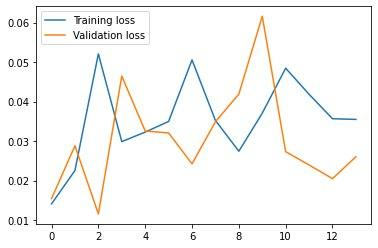
\includegraphics[width = 0.4 \textwidth]{random_curva_aprendizaje}
    \caption{Curva de aprendizaje para el entrenamiento del modelo usando triples aleatorios. En azul, la función de pérdida en entrenamiento. En naranja, la función de pérdida en validación}
\end{figure}

En dicha curva de aprendizaje se muetra un claro comportamiento errático en el aprendizaje. Esto puede deberse a los siguientes motivos:

\begin{itemize}
  \item El valor del \emph{learning rate} es demasiado alto y por eso el ajuste del error con \emph{back propagation} provoca dicho comportamiento errático
  \item No hemos entrenado durante suficientes épocas. Si entrenásemos durante más épocas, podríamos ver una tendencia global no tan errática
  \item El uso de triples aleatorios no es adecuado para optimizar la red, y por ello obtenemos dicho comportamiento errático
\end{itemize}

Comprobamos que no hemos usado pocas épocas entrenando durante 50, en vez de 10. La curva de aprendizaje en este caso es la siguiente:

\begin{figure}[H]
    \centering
    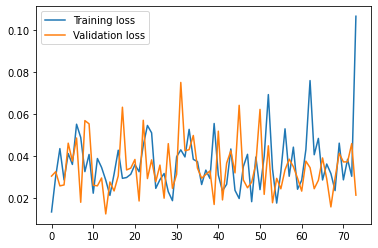
\includegraphics[width = 0.4 \textwidth]{random_curva_aprendizaje_larga}
    \caption{Curva de aprendizaje para el entrenamiento del modelo usando triples aleatorios. En este caso, en vez de entrenar durante 10 épocas, entrenamos durante 50}
\end{figure}

Seguimos observando el mismo comportamiento errático, y por tanto, descartamos que dicho comportamiento se explique por el uso de insuficientes épocas en el entrenamiento. Respecto al \emph{learning rate}, mostramos ahora el resultado de entrenar durante 10 épocas con un \emph{learning rate} mucho más bajo (en concreto, $0.0001$). La curva de aprendizaje en este caso es la siguiente:

\begin{figure}[H]
    \centering
    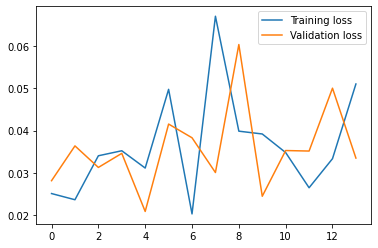
\includegraphics[width = 0.4 \textwidth]{random_curva_aprendizaje_lrbajo}
    \caption{Curva de aprendizaje para el entrenamiento del modelo usando triples aleatorios. En este caso, en vez de entrenar usando un \emph{learning rate} de 0.001, usamos 0.0001. De nuevo, estamos entrenando durante 10 épocas}
\end{figure}

El comportamiento errático sigue mostrándose con claridad. Por tanto, descartamos las dos primeras hipótesis para explicar el comportamiento errático, y consideramos la más probable la última: el uso de triples aleatorios no es adecuado para la optimización de la red.

Notar que en el \emph{Notebook} entregado usamos, tanto para el margen como para el \emph{learning rate} los parámetros originales. Si se quieren obtener los resultados que hemos mostrado para descartar hipótesis basta con modificar dichos parámetros en la celda con todos los hiperparámetros del \emph{Notebook}.

Obtenemos un valor de la función de pérdida, en el conjunto de test, de $0.0621$. Dicho valor se consigue usando la función \lstinline{test_model}, que se encuentra en nuestra librería, en el fichero \lstinline{core.py}. Más adelante, en \customcite{random_adaptacion_resultados_clasificacion:seccion}, mostraremos más métricas del modelo obtenido, una vez que lo hayamos adaptado a una tarea de clasificación.

\pagebreak

\subsection{Adaptación a una tarea de clasificación} 

Una vez entrenada la red, disponemos de una red que transforma imágenes en un espacio $\mathbb{R}^d$ con $d$ pequeña. Además, tenemos la propiedad fundamental que ya hemos comentado varias veces: imágenes de la misma clase tienen representaciones cercanas, e imágenes de clases distintas tienen representaciones lejanas.

Por ello, parece adecuado usar el algoritmo \emph{k-NN} para adaptar nuestra red, que simplemente calcula cierta representación de las imágenes, para una tarea de clasificación. Esto es lo que hacemos en la clase \lstinline{EmbeddingToClassifier}, que toma una red de este tipo y realiza la adaptación que ya hemos comentado.

Para ello, toma la red y el conjunto de imágenes que usaremos como base de instancias para \emph{k-NN}. Calculamos y almacenamos las representaciones de todas las imágenes. Cuando llega un nuevo ejemplo (una nueva imagen), calculamos su representación y aplicamos \emph{k-NN} sobre nuestro conjunto almacenado de representaciones. 

En nuestro caso, usaremos $k = 3$. Los resultados de realizar esta adaptación a la tarea de clasificación se muestran a continuación.

\pagebreak 

\subsubsection{Resultados de clasificación} \label{random_adaptacion_resultados_clasificacion:seccion}

Nos aprovechamos de los cálculos que realizamos en la adaptación del modelo a clasificación para mostrar la gráfica del \emph{embedding} obtenido sobre el conjunto de entrenamiento:

\begin{figure}[H]
    \centering
    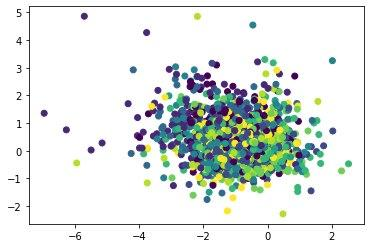
\includegraphics[width = 0.4 \textwidth]{random_embedding}
    \caption{Gráfica del \emph{embedding} calculado por la red sobre el conjunto de entrenamiento. Los colores muestran la clase asociada a cada uno de los puntos que mostramos}
\end{figure}

Como se puede ver en el gráfico anterior, las distintas clases se hallan muy juntas entre sí y entremezcladas, sin una separación clara por clase, por lo que la red no está separando correctamente las distintas clases del dataset. Este comportamiento era esperable debido a los malos resultados obtenidos previamente en el entrenamiento, y que mostrábamos en \customcite{resultados_entrenamiento:seccion}

Por otra parte, si ahora extraemos algunas métricas como son el Accurcy del clasificador, el Área bajo la curva ROC o la métrica Silohuette sobre el modelo de clasificación KNN obtenemos lo siguiente: 

\begin{table}[H]
\begin{center}
    \begin{tabular}{|c|c|c|c|}
        \hline
        Dataset & Accuracy & Área bajo la curva ROC & Silhouette \\
        \hline
        train & 0.125 & 0.5562 & -0.1894  \\
        test & 0.1042 & 0.5075 &  -0.1014 \\
        \hline
    \end{tabular}
\end{center}
    \caption{Métricas adicionales del modelo entrenado usando triples aleatorios}
\end{table}


Como podemos observar, el Accuracy obtenido tanto en entrenamiento como en test por el clasificador es muy bajo, de un 10\%. Por otro lado el Área bajo la curva ROC es de un 0.5, lo que nos indica que el comportamiento que tiene el clasificador es prácticamente aleatorio. Finalmente en la métrica Silohuette obtenemos un -0.1014 lo que nos indica que las fronteras de las distintas clases se encuentran entremezcladas, es decir, los elementos de las distintas clases no están bien separados unos de los otros. No obtenemos \emph{clusters} de calidad en el \emph{embedding} calculado.

En definitiva, estamos obteniendo unos resultados muy malos debido a una red que calcula un \emph{embedding} muy pobre. Como el algoritmo \emph{k-NN} depende fundamentalmente de la calidad de dicho \emph{embedding}, era de esperar, a la vista de los resultados de \customcite{resultados_entrenamiento:seccion}, un comportamiento muy malo en la adaptación a clasificación.

\pagebreak

\subsection{Conclusiones} \label{conclusiones_triples_aleatorios:seccion}

Los resultados obtenidos por el modelo de clasificación usando la Red Siamesa entrenada con triples aleatorios son muy pobres, como hemos mostrado tanto en \customcite{resultados_entrenamiento:seccion} como en \customcite{random_adaptacion_resultados_clasificacion:seccion}. Claramente no se pueden tomar como una solución al problema planteado en este proyecto. 

No obstante este modelo constituye un buen punto de partida sobre el cual mejorar los resultados obtenidos. En \customcite{resultados_entrenamiento:seccion} hemos defendido la hipótesis de que el comportamiento errático está causado por la inconveniencia de los triples aleatorios como mecanismo de selección de dichos triples. Por tanto, veremos más adelante si un mecanismo más adecuado de selección de triples consigue optimizar de forma correcta la red con la que estamos trabajando.

Cabe destacar de nuevo que no hemos realizado una exploración de los hiperparámetros que definen el modelo y su entrenamiento. Principalmente, el valor del margen para la función de pérdida, el \emph{learning rate} y la dimensión del \emph{embedding} resultante. No tenemos tiempo para realizar una exploración que requiere mucho tiempo de cómputo. Además, consideramos que este mal comportamiento no se va a corregir con una mejor selección de parámetros.

\pagebreak

\section{Entrenamiento usando triples \emph{online}}

\subsection{Detalles de implementación}

En este caso cambiaremos la estrategia para generar los triples (\emph{anchor}, \emph{positive}, \emph{negative}). Como el entrenamiento de la red se realiza por medio de mini batches, vamos a calcular para cada mini batch de imágnenes del dataset los triples más difíciles posibles. 

Entendemos por triple difícil aquel cuya distancia entre el \emph{anchor} y el \emph{positive} es el máximo de entre todas las distancias a los positivos del minibatch y la distancia entre el \emph{anchor} y \emph{negative} es el mínimo de entre todas las distancias a los negativos del minibatch.

A causa de este nuevo enfoque, resulta interesante el empleo de minibatches de gran tamaño (usaremos 1024) pues encontraremos conjuntos de triples más difíciles cuantas más imágenes haya en el minibatch.

Por otro lado aclarar que de esta forma, de un minibatch de 1024 imágenes del dataset, obtendremos como resultado un minibatch de 1024 triples difíciles que pasaremos a la red para entrenarla.

Finalmente el número de épocas establecidas para el entrenamiento es de 7.

\subsection{\emph{Hyperparameter tuning}} \label{hyperparameter_tuning:seccion}

\subsection{Resultados del entrenamiento}

\subsection{Adaptación a una tarea de clasificación}

De la misma forma que se hizo en el caso de triples aleatorios creamos un clasificador utilizando kNN con $k = 3$.

\subsection{Conclusiones}


\pagebreak

\section{Conclusiones}

\pagebreak

% Bibliografia
\bibliography{./References}
\bibliographystyle{ieeetr}

\end{document}
